\documentclass[]{report}

\voffset=-1.5cm
\oddsidemargin=0.0cm
\textwidth = 480pt

\usepackage{framed}
\usepackage{subfiles}
\usepackage{enumerate}
\usepackage{graphics}
\usepackage{newlfont}
\usepackage{eurosym}
\usepackage{amsmath,amsthm,amsfonts}
\usepackage{amsmath}
\usepackage{color}
\usepackage{amssymb}
\usepackage{multicol}
\usepackage[dvipsnames]{xcolor}
\usepackage{graphicx}
\begin{document}
\chapter{Set theory}



\section{Set Theory}
A set, in mathematics, is a collection of distinct entities, called its elements, considered as a whole. The early study of sets led to a family of paradoxes and apparent contradictions. It therefore became necessary to abandon "naïve" conceptions of sets, and a precise definition that avoids the paradoxes turns out to be a tricky matter. However, some unproblematic examples from naïve set theory will make the concept clearer. These examples will be used throughout this article:

\begin{itemize}
	\item A = the set of the numbers 1, 2 and 3.
	\item B = the set of primary light colours—red, green and blue.
	\item C = the empty set (the set with no elements).
	\item D = the set of all books in the British Library.
	\item E = the set of all positive integers, 1, 2, 3, 4, and so on.
\end{itemize}

Note that the last of these sets is infinite.

A set is the collection of its elements considered as a single, abstract entity. Note that this is different from the elements themselves, and may have different properties. For example, the elements of D are flammable (they are books), but D itself is not flammable, since abstract objects cannot be burnt.

\subsection{Notation - Listing Method}

By convention, a set can be written by \textbf{listing} its elements, separated by commas, between {braces}. 

Using the sets defined above:
\begin{itemize}
	\item A = $\{1, 2, 3\}$
	\item B = $\{red, green, blue\}$
	\item C = $\{\}$
\end{itemize}
This is impractical for large sets (D), and impossible for infinite ones (E). 
\subsection{Notation - Building Method}
Thus a set can also be described by naming a particular property that is shared by all its elements and only by them. A common notation uses a bar (|) to separate a variable name (e.g. "x") from a property of the variable that elements of the set must have. For example:
\begin{itemize}
	\item D = $\{x |$ x is a book and x is in the British Library $\}$
	\item E = $\{x |$ x is a positive integer$\}$
\end{itemize}
A simple translation of this notation is that "\textit{D is the set of all x, where x is a book and x is in the British Library}" or "\textit{E is the set of all x, where x is a positive integer}".

\section{Definition of a set}

A set is defined completely by its elements. Formally, sets X and Y are the same set if they have the same elements; that is, if every element of X is also an element of Y, and vice versa. For example, suppose we define:

\[ F = \{x | \mbox{(x is an integer)} \mbox{ and } 0 < x < 4)\}  \]
%Then F=A. The definition also makes it clear that {1,2,3} = (3,2,1} = {1,1,2,3,2}. Note also that if X and Y are both empty, then they are equal, justifying referring to "the" empty set.

The equivalence of empty sets has a \textbf{\textit{metaphysical}} consequence for some theories of the metaphysics of properties that define the property of being x as simply the set of all x, then if the two properties are uninstantiated or coextensive they are equivalent - under this theory, because there are no unicorns and there are no pixies, the property of being a unicorn and being a pixie are the same - but if there were a unicorns and pixies, we could tell them apart. (See Universals for more on this.)

\subsection{Elements and subsets}

The $\in$  sign indicates set membership. If x is an element (or "member") of a set X, we write $ \in X$; e.g. $3\in A$. (We may also say ``X contains x" and ``A contains 3")

A very important notion is that of a subset. X is a subset of Y, written $X \subseteq Y$ (sometimes simply as$X \subset Y$), if every element of X is also an element of Y. From before $C\subseteq A \subseteq E$.
\subsection{Sets containing Sets}


Sets can of course be elements of other sets; for example we can form the set $G = \{A,B,C,D,E\}$, whose five elements are the sets we considered earlier. Then, for instance, $A\in G$. (Note that this is very different from saying $A\subseteq G$)

%The tilde (~) is as usual used for negation; e.g. $\tilde(A\in B)$.

\subsection{Set operations}

Suppose X and Y are sets. Various operations allow us to build new sets from them.

\begin{description}
	\item[Union]
	The union of X and Y, written $X\cup Y$, contains all the elements in X and all those in Y. Thus $A \cup B = \{1, 2, 3, red, green, blue\}$. As A is a subset of E, the set $A \cup E$ is just E.
	
	\item[Intersection]
	
	The intersection of X and Y, written X∩Y, contains all the elements that are common to both X and Y. Thus {1,2,3,red,green,blue} ∩ {2,4,6,8,10} = {2}.
	
	\item[Set difference]
	
	The difference X minus Y, written X−Y or $X\|Y$, contains all those elements in X that are not also in Y. For example, E−A contains all integers greater than 3. A−B is just A; red, green and blue were not elements of A, so no difference is made by excluding them.
\end{description}

%---------------------------------%

\subsection{Important Operations in Set Theory}

\begin{itemize}
	\item Union ($\cup$) - also known as the OR operator. A union signifies a bringing together. The union of the sets A and B consists of the elements that are in either A or B.
	\item Intersection ($\cap$) - also known as the AND operator. An intersection is where two things meet. The intersection of the sets A and B consists of the elements that in both A and B.
	\item Complement ($^{c}$) - The complement of the set A consists of all of the elements in the universal set that are not elements of A.
\end{itemize}

%------------------------------------------------------------------------%
\begin{itemize}
	\item[2.a] Describe the following set by the listing method
	\[ \{ 2r+1 : r \in Z^{+} and r \leq 5  \} \]
	\item[2.b] Let A,B be subsets of the universal set U.
	
	
\end{itemize}
%------------------------------------------------------------------------%
\begin{itemize}
	\item[3.a]
	Let n be an element of the set $\{10, 11, 12, 13, 14, 15, 16, 17, 18, 19\}$,
	and p and q be the propositions:
	p : n is even, $q : n > 15$.
	Draw up truth tables for the following statements and find the values of n for
	which they are true:
	(i) $p \vee \neg q$
	(ii) $\neg p \wedge q$
\end{itemize}


%--------------------------------- %
\subsection{Universal Set and the Empty Set}
The first is the \textbf{\textit{universal set}}, typically denoted $U$. This set is all of the elements that we may choose from. This set may be different from one setting to the next. 

For example one universal set may be the set of real numbers whereas for another problem the universal set may be the whole numbers $\{0, 1, 2,\ldots\}$.

The other set that requires consideration is called the \textit{\textbf{empty set}}. The empty set is the unique set is the set with no elements. We write this as $\{ \}$ and denote this set by $\emptyset$.


%---------------------------------%
\section{Number Sets}
The font that the symbols are written in (i.e. $\mathbb{N}$, $\mathbb{R}$) is known as \textit{\textbf{blackboard font}}.
\begin{itemize}
	\item $\mathbb{N}$ Natural Numbers ($0,1,2,3$) 
	(Not used in the CIS102 Syllabus)
	\item $\mathbb{Z}$ Integers ($-3,-2,-1,0,1,2,3, \ldots$)
	\begin{itemize}
		\item[$\ast$] $\mathbb{Z}^{+}$ Positive Integers
		\item[$\ast$] $\mathbb{Z}^{-}$ Negative Integers
	\end{itemize}
	\item $\mathbb{Q}$ Rational Numbers
	\item $\mathbb{R}$ Real Numbers
\end{itemize}

%---------------------------------------------------- %
\begin{frame}
	\frametitle{Cardinality of a Set}
	\Large
	\vspace{-1cm}
	\begin{itemize}
		\item The cardinality of a set A is the number of elements in A, which is written as $|A|$.
		\item An element of a set is any one of the \textbf{distinct} objects that make up that set.
		
	\end{itemize}
\end{frame}
%---------------------------------------------------- %
%---------------------------------------------------- %
\begin{frame}
	\frametitle{Cardinality of a Set}
	\Large
	\vspace{-1cm}
	\begin{itemize}
		
		\item Note that this vertical-bar notation looks the same as absolute value notation, 
		but the meaning of cardinality is different from absolute value.
		
		\item In particular, absolute value operates on numbers (e.g., $|-4| = 4$) 
		while cardinality operates on sets (e.g., $|\{-4\}| = 1$).
	\end{itemize}
\end{frame}
%---------------------------------------------------- %
%---------------------------------------------------- %
\begin{frame}
	\frametitle{Examples of cardinality}
	\LARGE
	\vspace{-1cm}
	\textbf{Examples}
	\begin{itemize}
		\item[(i)] $|\{2,6,7\}|$
		\item[(ii)] $|\{5,6,5,2,2,6,5,1,1,1\}|$
		\item[(iii)] $|\{ \;\}| = 0$. %The empty set has no elements.
		\item[(iv)] $|\{\{1,2\},\{3,4\}\}| = 2$. 
		%In this case the two elements of $\{\{1,2\},\{3,4\}\}$ are themselves sets: $\{1,2\}$ and $\{3,4\}$.
	\end{itemize}
\end{frame}

%---------------------------------------------------- %
%---------------------------------------------------- %
\begin{frame}
	\frametitle{Examples of cardinality}
	\LARGE
	\vspace{-1cm}
	\textbf{Examples}
	\begin{itemize}
		\item[(i)] $|\{2,6,7\}| $
		\vspace{2cm}
		\item[(ii)] $|\{5,6,5,2,2,6,5,1,1,1\}| $
	\end{itemize}
\end{frame}

%---------------------------------------------------- %
%---------------------------------------------------- %
\begin{frame}
	\frametitle{Examples of cardinality}
	\LARGE
	\vspace{-1cm}
	\textbf{Examples}
	\begin{itemize}
		\item[(i)] $|\{2,6,7\}| = 3 $
		\vspace{2cm}
		\item[(ii)] $|\{5,6,5,2,2,6,5,1,1,1\}| = |\{1,2,5,6\}| $
	\end{itemize}
\end{frame}

%---------------------------------------------------- %
%---------------------------------------------------- %
\begin{frame}
	\frametitle{Examples of cardinality}
	\LARGE
	\vspace{-1cm}
	\textbf{Examples}
	\begin{itemize}
		\item[(i)] $|\{2,6,7\}| $
		\vspace{2cm}
		\item[(ii)] $|\{5,6,5,2,2,6,5,1,1,1\}| = |\{1,2,5,6\}| $
	\end{itemize}
\end{frame}

%---------------------------------------------------- %
%---------------------------------------------------- %
\begin{frame}
	\frametitle{Examples of cardinality}
	\LARGE
	\vspace{-1cm}
	\textbf{Examples}
	\begin{itemize}
		\item[(i)] $|\{2,6,7\}| = 3$
		\vspace{2cm}
		\item[(ii)] $|\{5,6,5,2,2,6,5,1,1,1\}| = |\{1,2,5,6\}| = 4$
	\end{itemize}
\end{frame}
%---------------------------------------------------- %
%---------------------------------------------------- %
\begin{frame}
	\frametitle{Examples of cardinality}
	\LARGE
	\vspace{-1cm}
	\textbf{Examples}
	\begin{itemize}
		\item[(iii)] $|\{ \; \}| $
		\vspace{2cm}
		\item[(iv)] $|\{\{1,2\},\{3,4\}\}| $.
	\end{itemize}
\end{frame}

%---------------------------------------------------- %
%---------------------------------------------------- %
\begin{frame}
	\frametitle{Examples of cardinality}
=
	\textbf{Examples}
	\begin{itemize}
		\item[(iii)] $|\{ \; \}| = 0$. \\ The empty set has no elements.
		\vspace{0.4cm} 
		\item[(iv)] $|\{\{1,2\},\{3,4\}\}| = 2$. \\ \vspace{0.4cm} In this case the two elements of $\{\{1,2\},\{3,4\}\}$ are themselves sets: $\{1,2\}$ and $\{3,4\}$.
	\end{itemize}
\end{frame}

%---------------------------------------------------------------------------%
\subsection{Complement and universal set}

The universal set (if it exists), usually denoted U, is a set of which everything conceivable is a member. In pure set theory, normally sets are the only objects considered (unlike here, where we have also considered numbers, colours and books, for example); in this case U would be the set of all sets. (Non-set objects, where they are allowed, are called 'urelemente' and are discussed below.)

In the presence of a universal set we can define X′, the complement of X, to be $U−X$. X′ contains everything in the universe apart from the elements of X. We could alternatively have defined it as

\[X′ = \{x | \tilde (x\in X)\}\]
and U as the complement of the empty set.

\subsection{Cardinality}

The cardinality $\|X\|$ of X is, roughly speaking, its size. The empty set has size 0, while B = $\{red, green, blue\}$ has size 3. 

This method of expressing cardinality works for finite sets but is not helpful for infinite ones. A more useful notion is that of two sets having the same size: if a direct one-to-one correspondence can be found between the elements of X and those of Y, they have the same size. 

Consider the sets, both infinite, of positive integers $\{1,2,3,4, \ldots\}$ and of even positive integers $\{2,4,6,8, \ldots\}$. One is a subset of the other. Nevertheless they have the same cardinality, as is shown by the correspondence mapping n in the former set to 2n in the latter. We can express this by writing $\|X\|$ = $\|Y\|$, or by saying that X and Y are "equinumerous".

\subsection{Power set}

The power set of X, $P(X)$, is the set whose elements are all the subsets of X. Thus \[P(A) = \{ \{\}, \{1\}, \{2\}, \{3\}, \{1,2\}, \{1,3\}, \{2,3\}, \{1,2,3\}\}\]. The power set of the empty set $P(\{\})$ = $\{\{\}\}$. 

Note that in both cases the cardinality of the power set is strictly greater than that of base set: No one-to-one correspondence exists between the set and its power set. 

%Cantor proved that this in fact holds for any set (Cantor's Theorem). This is obvious for a finite set, but Cantor's ingenious proof made no reference to the set being finite; the theorem holds even for infinite sets. This was a powerful generalisation of his previous discovery that different sizes of infinity exist.


\section*{Rules of Inclusion, Listing and Cardinality}
For each of the following sets, a set is specified by the rules of inclusion method and listing method respectively. Also stated is the cardinality of that data set.
\subsection*{Worked example 1}
\begin{itemize}
	\item $\{ x : x $ is an odd integer $ 5 \leq x \leq 17 \}$
	\item $x = \{5,7,9,11,13,15,17\}$
	\item The cardinality of set $x$ is 7.
\end{itemize}

\subsection*{Worked example 2}
\begin{itemize}
	\item $\{ y : y $ is an even integer $ 6 \leq y < 18 \}$
	\item $y = \{6,8,10,12,14,16\}$
	\item The cardinality of set $y$ is 6.
\end{itemize}

\subsection*{Worked example 3}
A perfect square is a number that has a integer value as a
square root. 4 and 9 are perfect squares ($\sqrt{4} = 2$,
$\sqrt{9} = 3$).
\begin{itemize}
	\item $\{ z : z $ is an perfect square $ 1 < z < 100 \}$
	\item $z = \{4,9,16,25,36,49,64,81\}$
	\item The cardinality of set $z$ is 8.
\end{itemize}


\subsection*{Exercises}
For each of the following sets, write out the set using the listing method.
Also write down the cardinality of each set.

\begin{itemize} 
	\item $\{ s : s $ is an negative integer $ -10 \leq s \leq 0 \}$
	\item $\{ t : t $ is an even number $ 1 \leq t \leq 20 \}$
	\item $\{ u : u $ is a prime number $ 1 \leq u \leq 20 \}$
	\item $\{ v : v $ is a multiple of 3 $ 1 \leq v \leq 20 \}$
\end{itemize}
%-------------------------------------------------% 

\section*{Power Sets}
\subsection*{Worked Example}
Consider the set $Z$:
\[ Z = \{ a,b,c\}  \]
\begin{itemize}
	\item[Q1] How many sets are in the power set of $Z$? 
	\item[Q2] Write out the power set of $Z$. 
	\item[Q3] How many elements are in each element set?
\end{itemize}
%----------------------------------------------%
\subsection*{Solutions to Worked Example}

\begin{itemize}
	
	
	\item[Q1] There are 3 elements in $Z$. So there is $2^3 = 8$ element sets contained in the power set.
	
	\item[Q2] Write out the power set of $Z$.
	\[ \mathcal{P}(Z) = \{ \{0\}, \{a\}, \{b\}, \{c\}, \{a,b\}, \{a,c\}, \{b,c\}, \{a,b,c\} \]
	
	\item[Q3]
	\begin{itemize}
		\item[*] One element set is the null set - i.e. containing no
		elements \item[$\bullet$] Three element sets have only elements \item[$\bullet$]
		Three element sets have two elements \item[$\bullet$] One element set
		contains all three elements \item[$\bullet$] 1+3+3+1=8
	\end{itemize}
\end{itemize}
\subsection*{Exercise}
For the set $Y = \{u,v,w,x\}$ , answer the questions from the
previous exercise


%------------------------------------------------------%

\section*{Complement of a Set}
%(2.3.1) 
Consider the universal set $U$ such that
\[U=\{2,4,6,8,10,12,15\} \]
For each of the sets $A$,$B$,$C$ and $D$, specify the complement sets.
\begin{center}
	\begin{tabular}{|c|c|}
		\hline
		Set & Complement\\
		\hline $A=\{4,6,12,15\}$ &
		$A^{\prime}=\{2,8,10\}$ \\ \hline $B=\{4,8,10,15\}$ & \\ \hline
		$C=\{2,6,12,15\}$ & \\ \hline $D=\{8,10,15\}$ & \\ \hline
		
	\end{tabular}
\end{center}
%-------------------------------------%
% Binary Operations on Sets (2.3.2)
% Union , Intersection, Symmetric Difference
% Set Difference



\section*{Set Operations}
Consider the universal set $U$ such that
\[U=\{1,2,3,4,5,6,7,8,9\} \] 
and the sets
\[A=\{2,5,7,9\} \] 
\[B=\{2,4,6,8,9\} \]

\begin{itemize}
	\item[(a)] $A-B$
	\item[(b)] $A \otimes B$
	\item[(c)] $A \cap B$
	\item[(d)] $A \cup B$
	\item[(e)] $A^{\prime} \cap B^{\prime}$
	\item[(f)] $A^{\prime} \cup B^{\prime}$
\end{itemize}


\section*{Venn Diagrams}

Draw a Venn Diagram to represent the universal set
$\mathcal{U} = \{0,1,2,3,4,5,6\}$ with subsets:\\
$A = \{2,4,5\}$\\
$B = \{1,4,5,6\}$\\

\noindent Find each of the following
\begin{itemize}
	\item[(a)] $A \cup B $
	\item[(b)] $A \cap B $
	\item[(c)] $A-B$
	\item[(d)] $B-A$
	\item[(e)] $A \otimes B$
\end{itemize}

\end{document}








%-------------------------------------% Ellipsis

When using Ellipsis, it should be clear what the pattern is

%-------------------------------------%


%-----------Reference to section 2.2.3 Power Sets




%-------------------------------------%

%----(Reference to Section 2.2.2 Cardinality)



%-------------------------------------% % Complement of a set


%--------------------------------------%
\subsection*{ Three Sets }

%- Section 2.3.5 %- Associative Law %- Distribution Law





%-------------------------------------% %- Section 3
Propositional Logic A statement is a declarative sentence that
is either true or false.
\begin{itemize}
	\item $\tilde q$ not q \item $p \vee q$ \item $p \wedge \tilde
	q$
\end{itemize}

%-------------------------------%
------------------------------------------------
Question 1


$\{ s :  s is an odd integer and 2 \leq s \leq 10 \}$
$\{ 2m :  m \element Z and 5 \leq m \leq 10 \}$
$\{ 2^t :  t \element Z and 0 \leq t \leq 5 \}$

------------------------------------------------
Question 2

\{12,13,14,15,16,17\}
{0,5,-5,10,-10,15,-15,.....\}
	{6,8,10,12,14,16,18\}
		Question 5
		
		-----------------------------------------------------
		
		
		--------------------------------------------
		
		Let A, B be subsets of the universal set \mathcal{U}.
		
		Use membership tables to prove De Morgan's Laws.
		
		---------------------------------------------
		Draw a venn diagram to show three subsets A,B and C of a universal set U intersecting in
		the most general way?
		How are sets $X$ and $Z$ related?
		Can you describe each of the subsets X,Y and Z in terms  of the
		sets A,B,C using the operations union intersection and set complement.
		
		Construct Membership tables for each of the sets
		(A-B) - C
		A-(B- C)
		
		(A-B) -C = A-(B-C)
		A
		
		
		
		\begin{itemize}
			\item[a.] (1 mark) Write out the sample space for the outcomes for both players A and B.
			\item[b.] (1 mark) Write out the sample space for the outcomes of C, where C is the difference of the two scores (i.e. B-A)
			\item[c.] (1 mark) Are the sample points for the sample space of C equally probable? Provide a brief justification for your answer.
		\end{itemize}
		
		%----------------------------------------------------------%
		\newpage
		\section*{Section B: Set Operations}
		\begin{itemize}
			\item[B.1] complement of A $A^{\prime}$
			\item[B.2] Union $A \cup B$
			\item[B.3] Intersection $A \cap B$
			\item[B.4] Relative Difference $A \otimes B$
			\item[A.5]
			\item[A.6]
			\item[A.7]
			\item[A.8]
		\end{itemize}
		\newpage
		
		
		\begin{itemize}
			\item Specifying Sets
			\item Listing Method
			\item Rules of Inclusion method
		\end{itemize}
		
		
		\begin{itemize}
			\item Subsets Notation of a subset
			\item Cardinality of a set
			\item Power of a set
		\end{itemize}
		
		\subsection*{Operation on Sets}
		
		\begin{itemize}
			\item The complement of Set
			\item Binary Operations
			\begin{itemize}
				\item Union
				\item Intersection
			\end{itemize}
			\item Membership tables
			\item Laws for Combining Sets
		\end{itemize}
		%----------------------------------------------------------%
		\subsection*{Membership Tables}
		Using membership tables
		\begin{tabular}{|ccc|c|c|c|}
			\hline
			% after \\: \hline or \cline{col1-col2} \cline{col3-col4} ...
			A & B & C & x & y & z \\\hline
			0 & 0 & 0 & 1 & 1 & 1 \\
			0 & 0 & 1 & 0 & 0 & 1 \\
			0 & 1 & 0 & 0 & 0 & 1 \\
			0 & 1 & 1 & 0 & 0 & 1 \\
			1 & 0 & 0 & 1 & 0 & 1 \\
			1 & 0 & 1 & 1 & 0 & 1 \\
			1 & 1 & 0 & 0 & 0 & 1 \\
			1 & 1 & 1 & 1 & 0 & 1 \\
			\hline
		\end{tabular}
		
		%----------------------------------------------------------%
		\section*{Section B: Hexadecimal Numbers}
		\begin{itemize}
			\item[B.1]
			\item[B.2]
			\item[B.3]
			\item[B.4]
			\item[B.5]
			\item[B.6]
			\item[B.7]
			\item[B.8]
		\end{itemize}
		\newpage
		
		
		\subsection*{Associative Laws}
		\[ (A \cup B) \cup C =  A \cup (B \cup C)  \]
		\[ (A \cap B) \cap C =  A \cap (B \cap C)  \]
		
		\subsection*{Distributive Laws}
		\[ (A \cup B) \cap C =  (A \cup B) \cap (A \cup C)  \]
		\[ (A \cap B) \cup C =  (A \cap B) \cup (A \cap C)  \]
		
		
		\[ (A \cup B) \cap B^{\prime} \]
		%----------------------------------------------------------%
		\section*{Section C: Real and Rational Numbers}
		\begin{itemize}
			\item[C.1]
			\item[C.2]
			\item[C.3]
			\item[C.4]
			\item[C.5]
			\item[C.6]
			\item[C.7]
			\item[C.8]
		\end{itemize}
		\newpage
		%----------------------------------------------------------%
		\newpage
		\section*{Formulae}
		\begin{itemize}
			
			
			
			
			\item Bayes' Theorem:
			\begin{equation*}
			P(B|A)=\frac{P\left(A|B\right) \times P(B) }{P\left( A\right) }.
			\end{equation*}
			
			
			
			\item Binomial probability distribution:
			\begin{equation*}
			P(X = k) = ^{n}C_{k} \times p^{k} \times \left( 1-p\right) ^{n-k}\qquad \left( \text{where}\qquad
			^{n}C_{k} =\frac{n!}{k!\left(n-k\right) !}. \right)
			\end{equation*}
			
			\item Poisson probability distribution:
			\begin{equation*}
			P(X = k) =\frac{m^{k}\mathrm{e}^{-m}}{k!}.
			\end{equation*}
		\end{itemize}
		
		%--------------------------------- %
\section*{The Universal Set and the Empty Set}
\begin{itemize}
	\item The first is the \textbf{\textit{universal set}}, typically denoted $U$. This set is all of the elements that we may choose from. This set may be different from one setting to the next. 
	
	\item For example one universal set may be the set of all real numbers, denoted $\mathbb{R}$, whereas for another problem the universal set may be the whole numbers $\{0, 1, 2,\ldots\}$.
	
	\item The other set that requires consideration is called the \textit{\textbf{empty set}}. The empty set is the unique set is the set with no elements. We write this as $\{ \}$ and denote this set by $\emptyset$.
\end{itemize}
%---------------------------------%
\section*{Number Sets}
The font that the following symbols are written in (i.e. $\mathbb{N}$, $\mathbb{R}$) is known as \textit{\textbf{blackboard font}}.
\begin{itemize}
	\item $\mathbb{N}$ Natural Numbers ($1,2,3,\ldots$) 
	%\textit{(Not used in the CIS102 Syllabus)}
	\item $\mathbb{Z}$ Integers ($-3,-2,-1,0,1,2,3, \ldots$)
	\begin{itemize}
		\item[$\bullet$] $\mathbb{Z}^{+}$ Positive Integers
		\item[$\bullet$] $\mathbb{Z}^{-}$ Negative Integers
		\item[$\bullet$] 0 is not considered as either positive or negative.
	\end{itemize}
	\item $\mathbb{Q}$ Rational Numbers
	\item $\mathbb{R}$ Real Numbers
	\item $\mathbb{C}$ Complex Numbers
\end{itemize}
%========================================================================================= %

\section*{Rules of Inclusion, Listing and Cardinality}
For each of the following sets, a set is specified by the rules of inclusion method and listing method respectively. Also stated is the cardinality of that data set.
\subsection*{Worked example 1}
\begin{itemize}
	\item $\{ x : x $ is an odd integer $ 5 \leq x \leq 17 \}$
	\item $x = \{5,7,9,11,13,15,17\}$
	\item The cardinality of set $x$ is 7.
\end{itemize}

\subsection*{Worked example 2}
\begin{itemize}
	\item $\{ y : y $ is an even integer $ 6 \leq y < 18 \}$
	\item $y = \{6,8,10,12,14,16\}$
	\item The cardinality of set $y$ is 6.
\end{itemize}

\subsection*{Worked example 3}
A perfect square is a number that has a integer value as a
square root. 4 and 9 are perfect squares ($\sqrt{4} = 2$,
$\sqrt{9} = 3$).
\begin{itemize}
	\item $\{ z : z $ is an perfect square $ 1 < z < 100 \}$
	\item $z = \{4,9,16,25,36,49,64,81\}$
	\item The cardinality of set $z$ is 8.
\end{itemize}

\newpage

\subsection*{Exercises}
For each of the following sets, write out the set using the listing method.
Also write down the cardinality of each set.

\begin{itemize} 
	\item $\{ s : s $ is an negative integer $ -10 \leq s \leq 0 \}$
	\item $\{ t : t $ is an even number $ 1 \leq t \leq 20 \}$
	\item $\{ u : u $ is a prime number $ 1 \leq u \leq 20 \}$
	\item $\{ v : v $ is a multiple of 3 $ 1 \leq v \leq 20 \}$
\end{itemize}
%-------------------------------------------------% 
\newpage
\section*{Power Sets}
\subsection*{Worked Example}
Consider the set $Z$:
\[ Z = \{ a,b,c\}  \]
\begin{itemize}
	\item[(i)] How many sets are in the power set of $Z$? 
	\item[(ii)] Write out the power set of $Z$. 
	\item[(iii)] How many elements are in each element set?
\end{itemize}
%----------------------------------------------%
\subsection*{Solutions to Worked Example}

\begin{itemize}
	
	
	\item[(i)] There are 3 elements in $Z$. So there is $2^3 = 8$ element sets contained in the power set.
	
	\item[(ii)] Write out the power set of $Z$.
	\[ \mathcal{P}(Z) = \{ \emptyset, \{a\}, \{b\}, \{c\}, \{a,b\}, \{a,c\}, \{b,c\}, \{a,b,c\} \} \]
	
	\item[(iii)]
	\begin{itemize}
		\item[$\bullet$] One element set is the null set - i.e. containing no
		elements \item[$\bullet$] Three element sets have only elements \item[$\bullet$]
		Three element sets have two elements \item[$\bullet$] One element set
		contains all three elements \item[$\bullet$] 1+3+3+1=8
	\end{itemize}
\end{itemize}
\subsection*{Exercise}
For the set $Y = \{u,v,w,x\}$ , answer the questions from the
previous exercise


%------------------------------------------------------%

\section*{Complement of a Set}
%(2.3.1) 
Consider the universal set $U$ such that
\[U=\{2,4,6,8,10,12,15\} \]
For each of the sets $A$,$B$,$C$ and $D$, specify the complement sets.
{
	
	\begin{center}
		\begin{tabular}{|c|c|}
			\hline
			Set &\phantom{sp} Complement \phantom{sp}\\
			\hline \phantom{sp} $A=\{4,6,12,15\}$ \phantom{sp} &
			$A^{\prime}=\{2,8,10\}$ \\ \hline $B=\{4,8,10,15\}$ & \\ \hline
			$C=\{2,6,12,15\}$ & \\ \hline $D=\{8,10,15\}$ & \\ \hline
			
		\end{tabular}
	\end{center}
}
%-------------------------------------%
% Binary Operations on Sets (2.3.2)
% Union , Intersection, Symmetric Difference
% Set Difference

%======================================================================================= %
\newpage



\subsection{Ellipsis}

When using Ellipsis, it should be clear what the pattern is

%-------------------------------------%


%-----------Reference to section 2.2.3 Power Sets




%-------------------------------------%

%----(Reference to Section 2.2.2 Cardinality)



%-------------------------------------% % Complement of a set


%--------------------------------------%
\subsection*{ Three Sets }

%- Section 2.3.5 %- Associative Law %- Distribution Law





%-------------------------------------% %- Section 3
Propositional Logic A statement is a declarative sentence that
is either true or false.
\begin{itemize}
	\item $\tilde q$ not q \item $p \vee q$ \item $p \wedge \tilde
	q$
\end{itemize}



%======================================================================================= %

Question 5


Let A, B be subsets of the universal set $\mathcal{U}$.

Use membership tables to prove De Morgan's Laws.


%
%Construct Membership tables for each of the sets
%(A-B) - C
%A-(B- C)
%
%(A-B) -C = A-(B-C)
%A
%


\begin{itemize}
	\item[a.] (1 mark) Write out the sample space for the outcomes for both players A and B.
	\item[b.] (1 mark) Write out the sample space for the outcomes of C, where C is the difference of the two scores (i.e. B-A)
	\item[c.] (1 mark) Are the sample points for the sample space of C equally probable? Provide a brief justification for your answer.
\end{itemize}

%----------------------------------------------------------%
\newpage
\section*{Section B: Set Operations}
\begin{itemize}
	\item[B.1] complement of A $A^{\prime}$
	\item[B.2] Union $A \cup B$
	\item[B.3] Intersection $A \cap B$
	\item[B.4] Relative Difference $A \otimes B$
	\item[A.5]
	\item[A.6]
	\item[A.7]
	\item[A.8]
\end{itemize}
\newpage


\begin{itemize}
	\item Specifying Sets
	\item Listing Method
	\item Rules of Inclusion method
\end{itemize}


\begin{itemize}
	\item Subsets Notation of a subset
	\item Cardinality of a set
	\item Power of a set
\end{itemize}

\subsection*{Operation on Sets}

\begin{itemize}
	\item The complement of Set
	\item Binary Operations
	\begin{itemize}
		\item Union
		\item Intersection
	\end{itemize}
	\item Membership tables
	\item Laws for Combining Sets
\end{itemize}

\newpage


\subsection*{Associative Laws}
\[ (A \cup B) \cup C =  A \cup (B \cup C)  \]
\[ (A \cap B) \cap C =  A \cap (B \cap C)  \]

\subsection*{Distributive Laws}
\[ (A \cup B) \cap C =  (A \cup B) \cap (A \cup C)  \]
\[ (A \cap B) \cup C =  (A \cap B) \cup (A \cap C)  \]


\[ (A \cup B) \cap B^{\prime} \]
%----------------------------------------------------------%
\section*{Section C: Real and Rational Numbers}

%----------------------------------------------------------%
\newpage
\section*{Formulae}
\begin{itemize}
	
	
	
	
	\item Bayes' Theorem:
	\begin{equation*}
	P(B|A)=\frac{P\left(A|B\right) \times P(B) }{P\left( A\right) }.
	\end{equation*}
	
	
	
	\item Binomial probability distribution:
	\begin{equation*}
	P(X = k) = ^{n}C_{k} \times p^{k} \times \left( 1-p\right) ^{n-k}\qquad \left( \text{where}\qquad
	^{n}C_{k} =\frac{n!}{k!\left(n-k\right) !}. \right)
	\end{equation*}
	
	\item Poisson probability distribution:
	\begin{equation*}
	P(X = k) =\frac{m^{k}\mathrm{e}^{-m}}{k!}.
	\end{equation*}
\end{itemize}

\section{Video 1 :  Set Theory Listing Method}
%--------------------------------------------%

%--------------------------------------------%

\section{Set Theory : Listing Method}

Describe the following sets using the Listing Method

\begin{itemize}
	\item[(i)] $ \{ 10^m : -2 \leq m \leq 4, m \in \mathbb{Z} \} $
	\item[(ii)]  $ \{ \frac{1}{n}: 1 < n < 4, n \in \mathbb{Z} \} $
\end{itemize}





\textbf{Part 1:} $ \{ 10^m : -2 \leq m \leq 4, m \in \mathbb{Z} \} $


%--------------------------------------------%

%\frametitle{Set Theory : Listing Method}

\textbf{Part 2:} $ \{ \frac{1}{n}: 1 < n < 4, n \in \mathbb{Z} \} $



\section*{Set Theory}

\begin{itemize}
\item[1.1] Introduction  
\item[1.2] Sets  
\item[1.3] Sub-sets  
\item[1.4] The order of sets: finite and infinite sets .
\item[1.5] Union and intersection of sets  
\item[1.6] Differences and complements  
\item[1.7] Venn diagrams  
\item[1.8] Logic analysis
\end{itemize}  
%-----------------------------------------------------%

\section{Specifying Sets}



\begin{enumerate}
	\item Listing Method
	\item Rules of Inclusion
\end{enumerate}

\subsection*{Part A : Builder Method}
The following sets have been defined using the \textbf{Building Method} of notation. Re-write them by listing \textbf{some} of the elements.
\begin{enumerate}
	\item $\{p | p$ is a capital city, p is in Europe$\}$
	\item $\{x | x = 2n - 5,$ x and n are natural numbers$\}$
	\item $\{y | 2y^2 = 50,$ y is an integer$\}$
	\item $\{z | z = n^3,$ z and n are natural numbers$\}$
\end{enumerate}
\subsection*{Part B : Sets}
U = {natural numbers}; $A = \{2, 4, 6, 8, 10\}$; $B = \{1, 3, 6, 7, 8\}$. State whether each of the following is true or false:
\begin{itemize}
	\item[(i)] $A \subset U$
	\item[(ii)] $B \subseteq A$
	\item[(iii)] $\emptyset \subset U$
\end{itemize}

%-------------------------------------- %

\begin{itemize}
	\item[\textbf{A}] $ \{ 2n : n \in \mathbb{Z^{+}} \} $
	\item[\textbf{B}] $ \{ 3,6,9,12,15,18,\ldots \} $
\end{itemize}
\textbf{Questions}
\begin{itemize}
	\item[(i)] \textbf{A} is described by the rules of inclusion. Describe \textbf{A} with the listing method.
	\item[(ii)] \textbf{B} is described by the listing method. Describe \textbf{B} with the rules of inclusion. 
\end{itemize}





\section{Set Theory Operations}
\begin{enumerate}
	\item The Universal Set $\mathcal{U}$
	\item Union
	\item Intersection
	\item Set Difference
	\item Relative Difference
\end{enumerate}




NOTATIONS FOR A SET:

A set can be represented by two methods:
1.ROSTER METHOD
2.BUILDER METHOD
ROSTER METHOD:

In this method the elements of a set are separated by commas and are enclosed within curly brackets { }. For example:

$A = {1, 2, 3, 4, 5, 6}$ is a set of numbers.

B = {Sunny, Joy, Kartik, Harish, Girish} is a set of names.

C = {a, e, i, o, u} is a set of vowels.

D = {apple, banana, guava, orange, pear} is a set of fruits.

Listing the elements in this way is called Roster method. In this method, it is not necessary for the elements to be listed in a particular order. The elements of the set can be written just plainly, separated by commas and in any order.


BUILDER METHOD:

This method is also called Property method. In Builder method, a set is represented by stating all the properties which are satisfied by the elements of that particular set only.

For example:

If A is a set of elements less than 0, then in Builder method it will be written as

$A = {x: x < 0}$, this statement is read as "the set of all x such that x is less than 0"

If A is a set of all real numbers less than 7, then in Builder method it is written as $A = {x   R: x < 7}$

Similarly,

$A = {2i: i is an integer}$ is a set of all even integers.

$A = {x   R: x \neq 2}$ is a set of all real numbers except 2.

$A = {x   R: x > 3 and x < 7}$ is a set of real numbers greater than 3 but less than 7.

$A = {x   Z: x > 6}$ is a set of integers greater than 6.

$A = {x   Z: 2x + 1}$ is a set of all odd integers.


\subsection{Set Theory Operations - Example}
%--------------------------------------------%

%\frametitle{Set Theory : Set Operations}

Given the following sets

\begin{center}
	\begin{tabular}{|c|c|} \hline
		$\mathcal{U}$ & $\{1,2,3,4,5,6,7,8,9\}$ \\ \hline
		$\mathcal{A}$ & $\{1,2,5,6,8\}$ \\ \hline
		$\mathcal{B}$ & $\{3,5,7,8\}$ \\ \hline
		$\mathcal{C}$ & $\{5,6,7,8,9\}$ \\ \hline
	\end{tabular}
\end{center}

List the elements of the following
$A^{\prime} \cap B $\\
$A^{\prime} \cap C $\\

%--------------------------------------------%


\subsection*{symbols}
$\varnothing$,
$\forall$,
$\in$,
$\notin$,
$\cup$
%----------------------------------------------------------- %

\subsection{Proper subset definition.} 
A proper subset of a set A is a subset of A that is not equal to A. In other words, if B is a proper subset of A, then all elements of B are in A but A contains at least one element that is not in B. For example, if A={1,3,5} then B={1,5} is a proper subset of A.



%---------------------------------------%


%%- Question 2B 2010 Zone A


\begin{itemize}
	\item Let A and B be subsets of the a universal set $U$.
	\item Use membership tables to prove that $(A \cup B^{\prime})^{\prime}$ = $A^{\prime} \cap B$
	\item Shade the regions corresponding to this set on a Venn Diagram
\end{itemize}

\begin{tabular}{|c|c|| c | c| c|}
	A&B&$B^{\prime}$&$A \cup B^{\prime}$&$(A \cup B^{\prime})^{\prime}$\\ \hline
	0&0&1&1&0\\
	0&1&0&0&1\\
	1&0&1&1&0\\
	1&1&0&1&0\\
\end{tabular}

\begin{tabular}{|c|c|| c | c| }
	A&B&$A^{\prime}$&$A^{\prime} \cap B$\\\hline
	0&0&1&0\\
	0&1&1&1\\
	1&0&0&0\\
	1&1&0&0\\
\end{tabular}



%-------------------------------------------%
% 2010 Zone A Q 1c
Given the universal set $U$ and subsets $A$ and $B$, list the set $(A \cup B^{\prime})^{\prime}$
\begin{itemize}
	\item $U=\{1,2,\ldots,8,9\}$
	\item $A=\{2,4,6,8\}$
	\item $B=\{ 4,5,6,7\}$
	\item $B^{\prime}=\{ 1, 2, 3, 8, 9  \}$
	\item $A \cup B^{\prime}=\{ 1, 2, 3,4, 6, 8, 9  \}$
	\item $(A \cup B^{\prime})^{\prime}=\{ 5,7 \}$
\end{itemize}




%----------------------------------------------------------------%

\section{Number Sets}

%% %% - \vspace{-1cm}
\textbf{Blackboard Bold Typeface}

\begin{itemize}
	\item Conventionally the symbols for numbers sets are written in a special typeface, known as \textbf{blackboard bold}.
	\item Examples : $\mathbb{N}$, $\mathbb{Z}$ and $\mathbb{R}$.
	
\end{itemize}


%% %% - \vspace{-1cm}
\textbf{Natural Numbers} ($\mathbb{N}$)
\begin{itemize}
	\item The whole numbers from 1 upwards. 
	
	\item The set of natural numbers is 
	\[\{1,2,3,4,5,6,\ldots\} \]
	\item In some branches of mathematics, $0$ might be counted as a natural number.
	\[\{0,1,2,3,4,5,6,\ldots\} \]
\end{itemize}

%----------------------------------------------------------------%


\subsection{Number Sets}


%% %% - \vspace{-0.5cm}
\textbf{Integers} ($\mathbb{Z}$)
\begin{itemize}
	\item The integers are all the whole numbers, all the negative whole numbers and zero.
	
	\item The set of integers is 
	\[\{\ldots,-4,-3,-2,-1,\;0,\;1,\;2,\;3,\ldots\} \]
	\item The notation $\mathbb{Z}$ is from the German word for numbers: \textit{Zahlen}. 
	\item All natural numbers are integers.
	\[ \mathbb{Q}  \subset \mathbb{Z}\]
\end{itemize}

%----------------------------------------------------------------%



%% %% - \vspace{-1.8cm}
\textbf{Integers} ($\mathbb{Z}$)
\begin{itemize}
	\item Natural numbers may also be referred to as positive integers, denoted $\mathbb{Z}^{+}$. \\(note the superscript)
	\item Negative integers are denoted $\mathbb{Z}^{-}$.
	\[\{\ldots,-4,-3,-2,-1\}\]
\end{itemize}

%----------------------------------------------------------------%

%% %% - \vspace{-1.8cm}
\textbf{Integers} ($\mathbb{Z}$)
\begin{itemize}
	\item 0 is neither positive nor negative. The following set of non-negative numbers \[\{0,1,2,3,4,5,6,\ldots\} \] might be denoted $0 \cup \mathbb{Z}^{+}$
	\item $\cup$ is the mathematical symbol for \textbf{union}.
\end{itemize}



%% %% - \vspace{-1cm}
\textbf{Rational Numbers} ($\mathbb{Q}$)
\begin{itemize}
	\item Rational numbers, also known as quotients, are numbers you can make by dividing one integer by another (but not dividing by zero). 
	\item If a number can be expressed as one integer divided by another, it is a rational number.
	\[ \mathbb{Q} = \left\{\; \frac{p}{q} \;\bigg| p \in \mathbb{Z},\; q \in \mathbb{Z},\; q \neq 0  \;   \right\}   \]
\end{itemize}

%-------------------------------------------------------------- %   


%% %% - \vspace{-1cm}
\textbf{Rational Numbers} ($\mathbb{Q}$)
\begin{itemize}
	\item All integers are rational numbers 
	\[ \mathbb{Z}  \subset \mathbb{Q}\]
	(and by extension all natural numbers are rational numbers too)
	\item Examples of rational numbers
	\[ 9500,\;7,\; \frac{1}{2} ,\; \frac{3}{7},\; -2.6 ,\; 0.001\] 
\end{itemize}

%-------------------------------------------------------------- %   

\subsection{Number Sets}

%% %% - \vspace{-1cm}
\textbf{Irrational Numbers} 
\begin{itemize}
	\item A number that can not be written as the ratio of two integers is known as an irrational number.
	\item Two famous examples of irrational numbers are $\pi$ and $\sqrt{2}$. 
	\[\pi = 3.141592\ldots\]
	\[\sqrt{2} = 1.41421\ldots\]
\end{itemize}

\textbf{Real Numbers} ($\mathbb{R}$)
\begin{itemize}
	\item Irrational numbers are types of real numbers.
	\item Rational numbers are real numbers too.
	\[ \mathbb{Q}  \subset \mathbb{R}\]
	
	\item A real number is simply any point anywhere on the number line.
\end{itemize}


\textbf{Real Numbers} ($\mathbb{R}$)
\begin{itemize}
	\item There are numbers that are not real numbers, for example \textbf{imaginary numbers}, but we will not cover them in this presentation.
\end{itemize}


%------------------------------------------$
2010 Zone B Q 1

5n+1 Rules of Inclusion method

$A = \{5n+1: n \in Z \}$

\subsection*{2011 Zone A question 1d}

Showing your workings, express the repeating decimal 0.012012012012...
as a rational number in its simplest form.


\begin{itemize}
	\item x = 0.012012012012...
	\item 10x = 0.12012012012... (not particularly useful )
	\item 100x = 1.2012012012... (not particularly useful either)
	\item 1000x= 12.012012012... (very useful)
	\item 999x = 12
	\item x= 12/999 = 4/333 (Answer!)
\end{itemize}

%------------------------------------------$

\subsection*{2008  Zone A question2a}
$B = \{3n-1 :n \in Z^{+} \}$
Describe the set B using the listing method

\begin{itemize}
	\item Let $n=1$. Consequently $3(1)-1 =2$
	\item Let $n=2$. Likewise $3(2)-1 =5$
	\item Let $n=3$. $3(3)-1 = 8 $
	\item The repeated differences are 3. The next few values are 11, 14 and 17
	\item So by the listing method $B= \{2,5,8,11,14,17,\ldots\}$
\end{itemize}

$A = \{3,5,7,9,ldots \}$
Describe the set A using the rules of inclusion method

\begin{itemize}
	\item The repeated differences are 2.
	\item We can say the rule has the form $2n+k$
	\item For the first value n=1. Therefore $2+k=3$
	\item Checking this , for the second value , n=2. Therefore $4+k=5$
	\item Clearly k = 1.
	\item $A = \{2n+1 :n \in Z^{+} \}$
	\item So by the listing method $B= \{2,5,8,11,14,17,\ldots\}$
\end{itemize}


\subsection{The Cartesian Product}
Exercises


Discrete Maths

A binary relation on a set A is the collection of ordered pairs of elements of A. In other words, it is the subset of the cartesian product A2= AA

Cartesian Product

This is a direct product pf 2 sets

XY = {(x,y)| xXandyY }

4 suits of cards and 13 Ranks, therefore 52 element cartesian prodcut.

N.B         AB BA
A=A =

Cartesian product is not associative
\subsection*{Worked Example}

Suppose that the Universal Set $\mathcal{U}$ is the set of integers from 1 to 9.
\[ \mathcal{U} = \{1,2,3,4,5,6,7,8,9\}, \]

and that the set $\mathcal{A}$ contains the prime numbers between 1 to 9 inclusive.

\[ \mathcal{A} = \{1,2,3,5,7\}, \]

and that the set $\mathcal{B}$ contains the even numbers between 1 to 9 inclusive.

\[ \mathcal{B} = \{2,4,6,8\}. \]

%--------------------------------------------------------%
\subsubsection*{Complements}
\begin{itemize}
	
	\item The Complements of A and B are the elements of the universal set not contained in A and B.
	
	\item The complements are denoted $\mathcal{A}^{\prime}$ and $\mathcal{B}^{\prime}$
	\[ \mathcal{A}^{\prime} = \{4,6,8,9\}, \]
	\[ \mathcal{B}^{\prime} = \{1,3,5,7,9\}, \]
	
\end{itemize}


%--------------------------------------------------------%

\subsubsection*{Intersection}
\begin{itemize}
	
	\item Intersection of two sets describes the elements that are members of both the specified Sets
	
	\item The intersection is denoted $\mathcal{A\cap B}$ 
	\[ \mathcal{A\cap B} = \{2\}\]
	
	\item only one element is a member of both A and B.
\end{itemize}
%--------------------------------------------------------%

\subsubsection*{Set Difference}
\begin{itemize}
	
	\item The Set Difference of A with regard to B are list of elements of A not contained by B.
	
	\item The complements are denoted $\mathcal{A-B}$ and $\mathcal{B-A}$
	\[ \mathcal{A-B} = \{1,3,5,7\}, \]
	
	\[ \mathcal{B-A} = \{4,6,8\}, \]
\end{itemize}

\subsection*{Union and intersection of sets}

\begin{itemize}
\item The \textbf{union} of two sets A and B is a set containing all the elements in
either A or B (or both)
i.e. 
\[A \cup B = {x / x \in A \mbox{ or } x \in B}.\]
\item The \textbf{intersection} of two sets A and B is a set containing all the elements
that are both in A and B
i.e. 
\[A \cap B = {x / x \in A \mbox{ and }x \in B}\].

\item If sets A and B have no elements in common, i.e. $A \cap B = \emptyset$,then A and B
are termed \textbf{disjoint sets}.
\end{itemize}

\subsection*{Subsets}

\begin{itemize}
\item Proper Subsets
\end{itemize}
\subsection*{The Power Set}




\section*{Question 2}
HibCollWorkSheet2

%Listing Method
%Rules of Inclusion
%Cardinality
%Venn diagrams

$\in$
$\subset$

univeral Set $\mathcal{U}$
Laws for Binary Operations
Membership Tables

De Morgan's Law


\[A^{\prime} \cup B^{\prime} = A \cap B\]



%--------------------------------------------------------%
\subsubsection*{Relative Difference}
\begin{itemize}
\item $ A \otimes B$
\end{itemize}
%--------------------------------------------------------%

\subsubsection*{Relative Difference}
\begin{itemize}
\item $ A \otimes B$
\end{itemize}
%--------------------------------------------------------%
\section{Power Sets}
\begin{itemize}
\item Consider the set A where $ A = \{w,x,y,z\}$
\item There are 4 elements in set A.
\item The power set of A contains 16 element data sets.
\item \[  \mathcal{P}(A) = \{\{ x \}, \{ y \} \}  \]
\item (i.e. 1 null set, 4 single element sets, 6 two -elemnts sets, 4 three lement set and one 4- element set.)
\end{itemize}
%------------------------------------------------%


%---------------------------- %
%---------------------------------------%
\subsubsection*{Power Sets}
\begin{itemize}
	\item Consider the set A where $ A = \{w,x,y,z\}$
	\item There are 4 elements in set A.
	\item The power set of A contains 16 element data sets.
	\item \[  \mathcal{P}(A) = \{\{ x \}, \{ y \} \}  \]
	\item (i.e. 1 null set, 4 single element sets, 6 two -elemnts sets, 4 three lement set and one 4- element set.)
\end{itemize}


%--------------------------------------------------------%
\subsection*{Dice Rolls}
Consider rolls of a die. What is the universal set?

\[ \mathcal{U} = \{1,2,3,4,5,6\} \]

%--------------------------------------%
\subsection*{Worked Example}

Suppose that the Universal Set $\mathcal{U}$ is the set of integers from 1 to 9.
\[ \mathcal{U} = \{1,2,3,4,5,6,7,8,9\}, \]

and that the set $\mathcal{A}$ contains the prime numbers between 1 to 9 inclusive.

\[ \mathcal{A} = \{1,2,3,5,7\}, \]

and that the set $\mathcal{B}$ contains the even numbers between 1 to 9 inclusive.

\[ \mathcal{B} = \{2,4,6,8\}. \]

%--------------------------------------------------------%
\subsubsection*{Complements}
\begin{itemize}

\item The Complements of A and B are the elements of the universal set not contained in A and B.

\item The complements are denoted $\mathcal{A}^{\prime}$ and $\mathcal{B}^{\prime}$
\[ \mathcal{A}^{\prime} = \{4,6,8,9\}, \]
\[ \mathcal{B}^{\prime} = \{1,3,5,7,9\}, \]

\end{itemize}


%--------------------------------------------------------%

\subsubsection*{Intersection}
\begin{itemize}

\item Intersection of two sets describes the elements that are members of both the specified Sets

\item The intersection is denoted $\mathcal{A\cap B}$ 
\[ \mathcal{A\cap B} = \{2\}\]

\item only one element is a member of both A and B.
\end{itemize}
%--------------------------------------------------------%

\subsubsection*{Set Difference}
\begin{itemize}

\item The Set Difference of A with regard to B are list of elements of A not contained by B.

\item The complements are denoted $\mathcal{A-B}$ and $\mathcal{B-A}$
\[ \mathcal{A-B} = \{1,3,5,7\}, \]

\[ \mathcal{B-A} = \{4,6,8\}, \]
\end{itemize}


%------------------------------------------$

\subsection*{2008  Zone A question2a}
$B = \{3n-1 :n \in Z^{+} \}$
Describe the set B using the listing method

\begin{itemize}
\item Let $n=1$. Consequently $3(1)-1 =2$
\item Let $n=2$. Likewise $3(2)-1 =5$
\item Let $n=3$. $3(3)-1 = 8 $
\item The repeated differences are 3. The next few values are 11, 14 and 17
\item So by the listing method $B= \{2,5,8,11,14,17,\ldots\}$
\end{itemize}

$A = \{3,5,7,9,ldots \}$
Describe the set A using the rules of inclusion method

\begin{itemize}
\item The repeated differences are 2.
\item We can say the rule has the form $2n+k$
\item For the first value n=1. Therefore $2+k=3$
\item Checking this , for the second value , n=2. Therefore $4+k=5$
\item Clearly k = 1.
\item $A = \{2n+1 :n \in Z^{+} \}$
\item So by the listing method $B= \{2,5,8,11,14,17,\ldots\}$
\end{itemize}

\section{Cartesian Product}

\begin{itemize}
\item Let $X$ and $Y$ be sets.
\item The \textbf{cartesian product} $X \times Y$ is the set whose elements are \textbf{all} of 
the ordered pairs of elements $(x,y)$ where $x \in X$ and $y \in Y$.
\end{itemize}

\begin{itemize}
\item Let $X = \{a,b,c\}$
\item Let $Y = \{0,1\}$ 
\item The cartesian product $X \times Y$ is therefore:
\end{itemize}

\begin{itemize}
\item Importantly $X \times Y \neq Y \times X$
\item Recall: Let $X = \{a,b,c\}$ and let $Y = \{0,1\}$ 
\item The cartesian product $Y \times X$ is therefore:
\end{itemize}






\subsection{The Cartesian Product}
Exercises


 Discrete Maths
 
A binary relation on a set A is the collection of ordered pairs of elements of A. In other words, it is the subset of the cartesian product A2= AA

Cartesian Product
 
This is a direct product pf 2 sets
 
XY = {(x,y)| xXandyY }
 
4 suits of cards and 13 Ranks, therefore 52 element cartesian prodcut.
 
N.B         AB BA
              A=A =
 
Cartesian product is not associative
\subsection*{Worked Example}

Suppose that the Universal Set $\mathcal{U}$ is the set of integers from 1 to 9.
\[ \mathcal{U} = \{1,2,3,4,5,6,7,8,9\}, \]

and that the set $\mathcal{A}$ contains the prime numbers between 1 to 9 inclusive.

\[ \mathcal{A} = \{1,2,3,5,7\}, \]

and that the set $\mathcal{B}$ contains the even numbers between 1 to 9 inclusive.

\[ \mathcal{B} = \{2,4,6,8\}. \]

%--------------------------------------------------------%
\subsubsection*{Complements}
\begin{itemize}

\item The Complements of A and B are the elements of the universal set not contained in A and B.

\item The complements are denoted $\mathcal{A}^{\prime}$ and $\mathcal{B}^{\prime}$
\[ \mathcal{A}^{\prime} = \{4,6,8,9\}, \]
\[ \mathcal{B}^{\prime} = \{1,3,5,7,9\}, \]

\end{itemize}


%--------------------------------------------------------%

\subsubsection*{Intersection}
\begin{itemize}

\item Intersection of two sets describes the elements that are members of both the specified Sets

\item The intersection is denoted $\mathcal{A\cap B}$ 
\[ \mathcal{A\cap B} = \{2\}\]

\item only one element is a member of both A and B.
\end{itemize}
%--------------------------------------------------------%

\subsubsection*{Set Difference}
\begin{itemize}

\item The Set Difference of A with regard to B are list of elements of A not contained by B.

\item The complements are denoted $\mathcal{A-B}$ and $\mathcal{B-A}$
\[ \mathcal{A-B} = \{1,3,5,7\}, \]

\[ \mathcal{B-A} = \{4,6,8\}, \]
\end{itemize}


\end{document}
\section*{Question 2}
Describe the following set by the rules of inclusion method.

Describe the following set by the listing method
the set of positive multiples of 3 which are less than 20.

Let A and B be subsets of univerisal set U

Use the membership rule to prove that

\[(A^\prime  \cap B)^\prime = A \cup B^\prime\]

shade the region corresponding to this set on a Venn Diagram

Given the universal set $\mathcal{U} = {1,2,3,4,5,6,7,8,9}$
and the subsets $A=\{1,3,5,7\}$
$B = \{6,7,8,9\}$
list the set $A^\prime \cap B)^\prime$ 



\begin{itemize}
\item[(i)] $\{5,8\}$
\item[(ii)] $\{1,2,3,4,5,6,7,8,9\}$ 
\end{itemize}

\section*{Set Operations}
\begin{itemize}
\item Union ($\cup$) - also known as the \textbf{OR} operator. A union signifies a bringing together. The union of the sets A and B consists of the elements that are in either A or B.
\item Intersection ($\cap$) - also known as the \textbf{AND} operator. An intersection is where two things meet. The intersection of the sets A and B consists of the elements that in both A and B.
\item Complement ($A^{\prime}$ or $A^{c}$) - The complement of the set A consists of all of the elements in the universal set that are not elements of A.
\end{itemize}

\subsection*{Exercise}
Consider the universal set $U$ such that
\[U=\{1,2,3,4,5,6,7,8,9\} \] 
and the sets
\[A=\{2,5,7,9\} \] 
\[B=\{2,4,6,8,9\} \]

\begin{multicols}{2}
\begin{itemize}
\item[(a)] $A-B$
\item[(b)] $A \otimes B$
\item[(c)] $A \cap B$
\item[(d)] $A \cup B$
\item[(e)] $A^{\prime} \cap B^{\prime}$
\item[(f)] $A^{\prime} \cup B^{\prime}$
\end{itemize}
\end{multicols}

%======================================================================================= %
\newpage

\section*{Venn Diagrams}

Draw a Venn Diagram to represent the universal set
$\mathcal{U} = \{0,1,2,3,4,5,6\}$ with subsets:\\
$A = \{2,4,5\}$\\
$B = \{1,4,5,6\}$\\

\noindent Find each of the following
\begin{itemize}
\item[(a)] $A \cup B $
\item[(b)] $A \cap B $
\item[(c)] $A-B$
\item[(d)] $B-A$
\item[(e)] $A \otimes B$
\end{itemize}
\newpage



%------------------------------------------------------------------------%
\begin{itemize}
\item[(i)] Describe the following set by the listing method
\[ \{ 2r+1 : r \in Z^{+} and r \leq 5  \} \]
\item[(ii)] Let A,B be subsets of the universal set U.


\end{itemize}

%===================================================================================== %
\subsection*{Question 1}

\begin{itemize}
\item $\{ s :  \mbox{ s is an odd integer and } 2 \leq s \leq 10 \}$
\item $\{ 2m :  m \in Z \mbox{ and }5 \leq m \leq 10 \}$
\item $\{ 2^t :  t \in Z \mbox{ and } 0 \leq t \leq 5 \}$
\end{itemize}

%=======================+============================================================== %
\subsection*{Question 2}

\begin{itemize}
\item $\{12,13,14,15,16,17\}$
\item $\{0,5,-5,10,-10,15,-15,.....\}$
\item $\{6,8,10,12,14,16,18\}$
\end{itemize}

\subsection*{Question 7 : Membership Tables}
Using membership tables
\begin{tabular}{|ccc|c|c|c|}
\hline
% after \\: \hline or \cline{col1-col2} \cline{col3-col4} ...
A & B & C & x & y & z \\\hline
0 & 0 & 0 & 1 & 1 & 1 \\
0 & 0 & 1 & 0 & 0 & 1 \\
0 & 1 & 0 & 0 & 0 & 1 \\
0 & 1 & 1 & 0 & 0 & 1 \\
1 & 0 & 0 & 1 & 0 & 1 \\
1 & 0 & 1 & 1 & 0 & 1 \\
1 & 1 & 0 & 0 & 0 & 1 \\
1 & 1 & 1 & 1 & 0 & 1 \\
\hline
\end{tabular}
\begin{itemize}
\item[(i)] Draw a venn diagram to show three subsets A,B and C of a universal set U intersecting in
the most general way?
\item[(ii)] How are sets $X$ and $Z$ related?
\item[(iii)] Can you describe each of the subsets X,Y and Z in terms  of the
sets A,B,C using the operations union intersection and set complement.
\end{itemize}
%================================================================ %
\section*{Question 4}
\[ \mbox{Log}_4 64 + \mbox{Log}_5 625 + \mbox{Log}_9 3 \] 


%------------------------------------%
\section*{Question 5}
\begin{enumerate}
\item Draw two non-isomorphic graphs with the following degree sequence.
\[ 4,3,3,2,2,2,2,1,1\]
\item
\end{enumerate}
%------------------------------------%

\section*{Question 7b}

Compute the following summation

\[ \sum^{i=100}_{i=25} i^2 + 3i -5)\]


%------------------------------------%

\section*{Section 2. Set Theory}


\subsection*{Membership Tables}
For the following venn diagrams, complete the membership.

The events $W$, $X$,$Y$ and $Z$ correspond to the shaded areas in each of the venn diagrams.


%------------------------------------------------------------------------%

\section{Subsets and the Power Set} (2.2)
Subsets and Proper Subsets
Cardinality of a Set
Power Set


%------------------------------------------------------------------------%

\section{Set operations (2.3)}

complement
union 
intersection
set difference


\section*{Venn Diagrams}

Subsets of the universal set $\mathcal{U}$, intersecting in the most general way (Essentially this means - the venn diagram allows for all possible combinations of overlap.)

\begin{center}
	\begin{tabular}{|c|c|}
		\hline  &  \\ 
		\hline  &  \\ 
		\hline 
	\end{tabular} 
\end{center}

%-------------------------- %
%-------------------------- %
%Section 3

\subsection*{Venn Diagrams}
%\begin{figure}
%\centering
%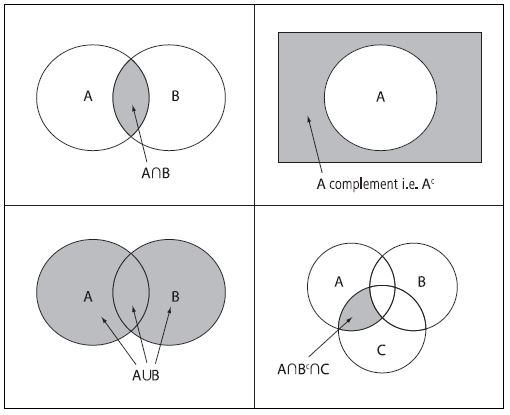
\includegraphics[width=0.7\linewidth]{venndiagram}
%
%\end{figure}
\[ \mbox{IMAGE}\]

%----------------------------------------%
%------------------------------------------------------------------------%

\section{Venn Diagrams}

venn diagrams
8 Disjoint Regions

%------------------------------------------------------------------------%
\subsection{Cartesian Product}
{
	\begin{itemize}
		\item Let $X$ and $Y$ be sets.
		\item The \textbf{cartesian product} $X \times Y$ is the set whose elements are \textbf{all} of 
		the ordered pairs of elements $(x,y)$ where $x \in X$ and $y \in Y$.
	\end{itemize}
	
	\begin{itemize}
		\item Let $X = \{a,b,c\}$
		\item Let $Y = \{0,1\}$ 
		\item The cartesian product $X \times Y$ is therefore:
	\end{itemize}
	
	\begin{itemize}
		\item Importantly $X \times Y \neq Y \times X$
		\item Recall: Let $X = \{a,b,c\}$ and let $Y = \{0,1\}$ 
		\item The cartesian product $Y \times X$ is therefore:
	\end{itemize}
}





\section{Sets of Numbers}

\begin{itemize}
\item $\mathbb{Z}$ Set of all integers
\item $\mathbb{Q}$ Set of all rational numbers
\item $\mathbb{R}$ Set of all real numbers
\end{itemize}


\begin{itemize}
\item $\mathbb{Z}^{+}$ Set of all positive integers
\item $\mathbb{Z}^{-}$ Set of all negative integers
\item $\mathbb{R}^{+}$ Set of all positive real numbers
\item $\mathbb{R}^{-}$ Set of all negative real numbers
\end{itemize}

%------------------------------------------------------------------------%
\end{document}
